%%%%%%%%%%%%%%%%%%%%%%%%%%%%%%%%%%%%%%%%%


\documentclass{beamer}

\mode<presentation> {


\usetheme{Madrid}




\usepackage{graphicx} 
\usepackage{booktabs} 
\usepackage{amsmath,amsfonts,amssymb}
\usepackage{mathtools}
\usepackage{nccmath}
}

\title[Short title]{Introduction to AI  and ML }

\author{Ujjwal (ee18btech11010), Pranay (ee18btech11009)}
\institute[IITH] 
{
Indian Institute of Technology\\ 
\medskip
\textit{Hyderabad}
}
\date{February 14, 2019}

\begin{document}
\begin{frame}
\titlepage 
\end{frame}

\begin{frame}
\frametitle{IIT JEE, 1980 (Geometric form)} 
Q. The point (4 , 1) undergoes the following three transformations successively .
\begin{enumerate}
\item    Reflection about the line y = x.
\item    Translation through a distance 2 units along the positive direction of x-axis .
\item Rotation through an angle  $ \frac{\pi}{4} $  about the origin in the counter clockwise direction.
\end{enumerate}

\end{frame}


%-----------------------------------------------------------------------------------
\begin{frame}
\frametitle{IIT JEE  mains, 1980 (Matrix form)} 
Q. The point   $ \begin{bmatrix} x \\y \end{bmatrix}  = \begin{bmatrix} 4 \\1 

\end{bmatrix} $
 undergoes the following three transformations successively .
\begin{enumerate}
\item    Reflection about the line $ \begin{bmatrix} 1 & -1 \end{bmatrix} \begin{bmatrix} x \\y \end{bmatrix}  = 0 $
\item    Translation through a distance 2 units along the positive direction of x-axis .
\item Rotation through an angle $\frac{\pi}{4} $ about the origin in the counter clockwise direction.
\end{enumerate}

\end{frame}

%------------------------------------------------
\begin{frame}
\frametitle{Graph}
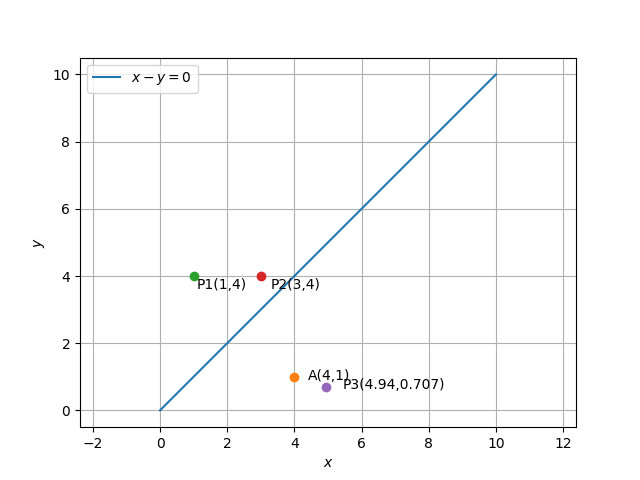
\includegraphics[height=8cm , width=12cm]{line}
\end{frame}
\begin{frame}
\frametitle{Solution}
Let the given point be A (4,1) be represented as,  \[A = \begin{bmatrix} 4\\ 1 

\end{bmatrix}\] \\
 Now, the first transformation is reflection about the line $y = x$.\\
 So , the matrix associated with this reflection is given by ,\\
 \[Z_{ref} =\begin{bmatrix} 0 & 1 \\ 1 & 0  \end{bmatrix}\] \\ Right multiplication of any matrix ,
 $A= \begin{bsmallmatrix} x\\y \end{bsmallmatrix}$ with Z is equivalent \break to the reflection of the point A(x,y) with respect to the given line,  $\begin{bmatrix} 1 & -1 \end{bmatrix} \begin{bmatrix} x \\y \end{bmatrix}  = 0 $ .
\end{frame}

%------------------------------------------------

\begin{frame}
\frametitle{Solution.}
So, we have A transformed to $P_{1}$ ,where\\
\quad \quad \quad \quad \quad \quad $ P_1 = Z_{ref}A = \begin{bmatrix} 0 & 1  \\ 1 & 0 \end{bmatrix}  \begin{bmatrix} x \\y \end{bmatrix} = \begin{bmatrix} 1 \\4 \end{bmatrix} $

\end{frame}

%------------------------------------------------------------
\begin{frame} 
\frametitle{Solution..}
The next transformation is shifting the point '$P_{1}$' by 2 units to \break the positive x-axis\\
Let $Q=  \begin{bsmallmatrix} 2\\0 \end{bsmallmatrix} $ be the column matrix associated with the current transformation.\\
After applying the transformation , the new transformed matrix $P_{2} $ corresponding to the point Q is ,\\
\quad \quad \quad\quad $P_2 = Q + P_1 = \begin{bmatrix} 2\\0 \end{bmatrix}  + \begin{bmatrix} 1\\4 \end{bmatrix} = \begin{bmatrix} 3\\4 \end{bmatrix}   $


\end{frame}

\begin{frame}
\frametitle{Solution...}

Now, the last transformation is rotating the point $P_{2}$ by  an \break angle  \(\frac{\pi}{4} \) in the counter clockwise direction about the origin.\\
Now, we have the \break rotation matrix,where $\theta$ is the angle of the rotation of the \break point  about the origin.

\[Z_{rotate} = \begin{bmatrix} \cos{\theta} & -\sin{\theta} \\ \sin{\theta} & \cos{\theta}\end{bmatrix}\]
\\Now, substituting $ \theta = \frac{\pi}{4}$
\[Z_{rotate} = \begin{bmatrix} 1/\sqrt{2} & -1/\sqrt{2} \\ 1/\sqrt{2} & 1/\sqrt{2}\end{bmatrix}\]

    
    
\end{frame}
\begin{frame}
 Right multiplication of the matrix ,
 $P_{2}= \begin{bsmallmatrix} x\\y \end{bsmallmatrix}$ with  $Z_{rotate}$  is equivalent \break to the rotation  of the point  $ P_{2}$ by an angle $ \theta$ about the origin.\\
    So, we have $P_{2} $ transformed to $P_{3}$ , where \\
    \[P_{3} = Z_{rotate}P_{2} = \begin{bmatrix} 1/\sqrt{2} & -1/\sqrt{2} \\ 1/\sqrt{2} & 1/\sqrt{2}\end{bmatrix} \begin{bmatrix} 3 \\4 \end{bmatrix} = \begin{bmatrix} -1/\sqrt{2} \\7/\sqrt{2} \end{bmatrix}  \]\\
    Therefore the final transformed matrix is ,
    \[P_{3} =\begin{bmatrix} -1/\sqrt{2} \\7/\sqrt{2} \end{bmatrix}  \]\\ 
    Hence, A(4,1) transforms to $ P_{3}(  \frac{-1}{\sqrt{2}}, \frac{7}{\sqrt{2}} )$
\end{frame}

\begin{frame}
\quad\quad\quad  \quad\quad\quad\quad\quad\quad \quad\quad\quad \quad\quad  THE END
\end{frame}
\end{document}